% Wang2025-focused single-RF insert generated from the 2026-07-09 focused matrix.
% Source tables: ../../06_analysis/paper_tables/wang2025_focused_single_rf_20260709/
% Source figures: ../../06_analysis/paper_figures/wang2025_focused_single_rf_20260709/

\subsection{Comparison Under a Wang-Style MIMO-OTFS FANET Matrix}
\label{subsec:wang_focused_matrix}

To separate the link-layer discovery contribution from the long-horizon MARL
transfer setting, we further evaluate the proposed budgeted ISAC access rule in
a Wang-style FANET matrix.  The setting follows the MIMO-OTFS sensing
abstraction used in the reference experiment: approximately 25-degree beams
(\(15\) azimuth cells and \(7\) elevation cells), a single RF chain, \(N\in
\{10,20,30,40,50\}\) UAVs, 200 discovery slots, five paired episodes per case,
and a single-hop communication/sensing range covering the 10 km cubic region.
The compared protocols are uniform random scanning, Wang-style ISAC without
table exchange, Wang-style communication-table exchange, Wang-style sensing-table
exchange, the non-budgeted ISAC rule, and the proposed budgeted ISAC access rule.
This experiment uses a PHY-aware sensing abstraction rather than a full
waveform receiver implementation.

\begin{figure}[!t]
  \centering
  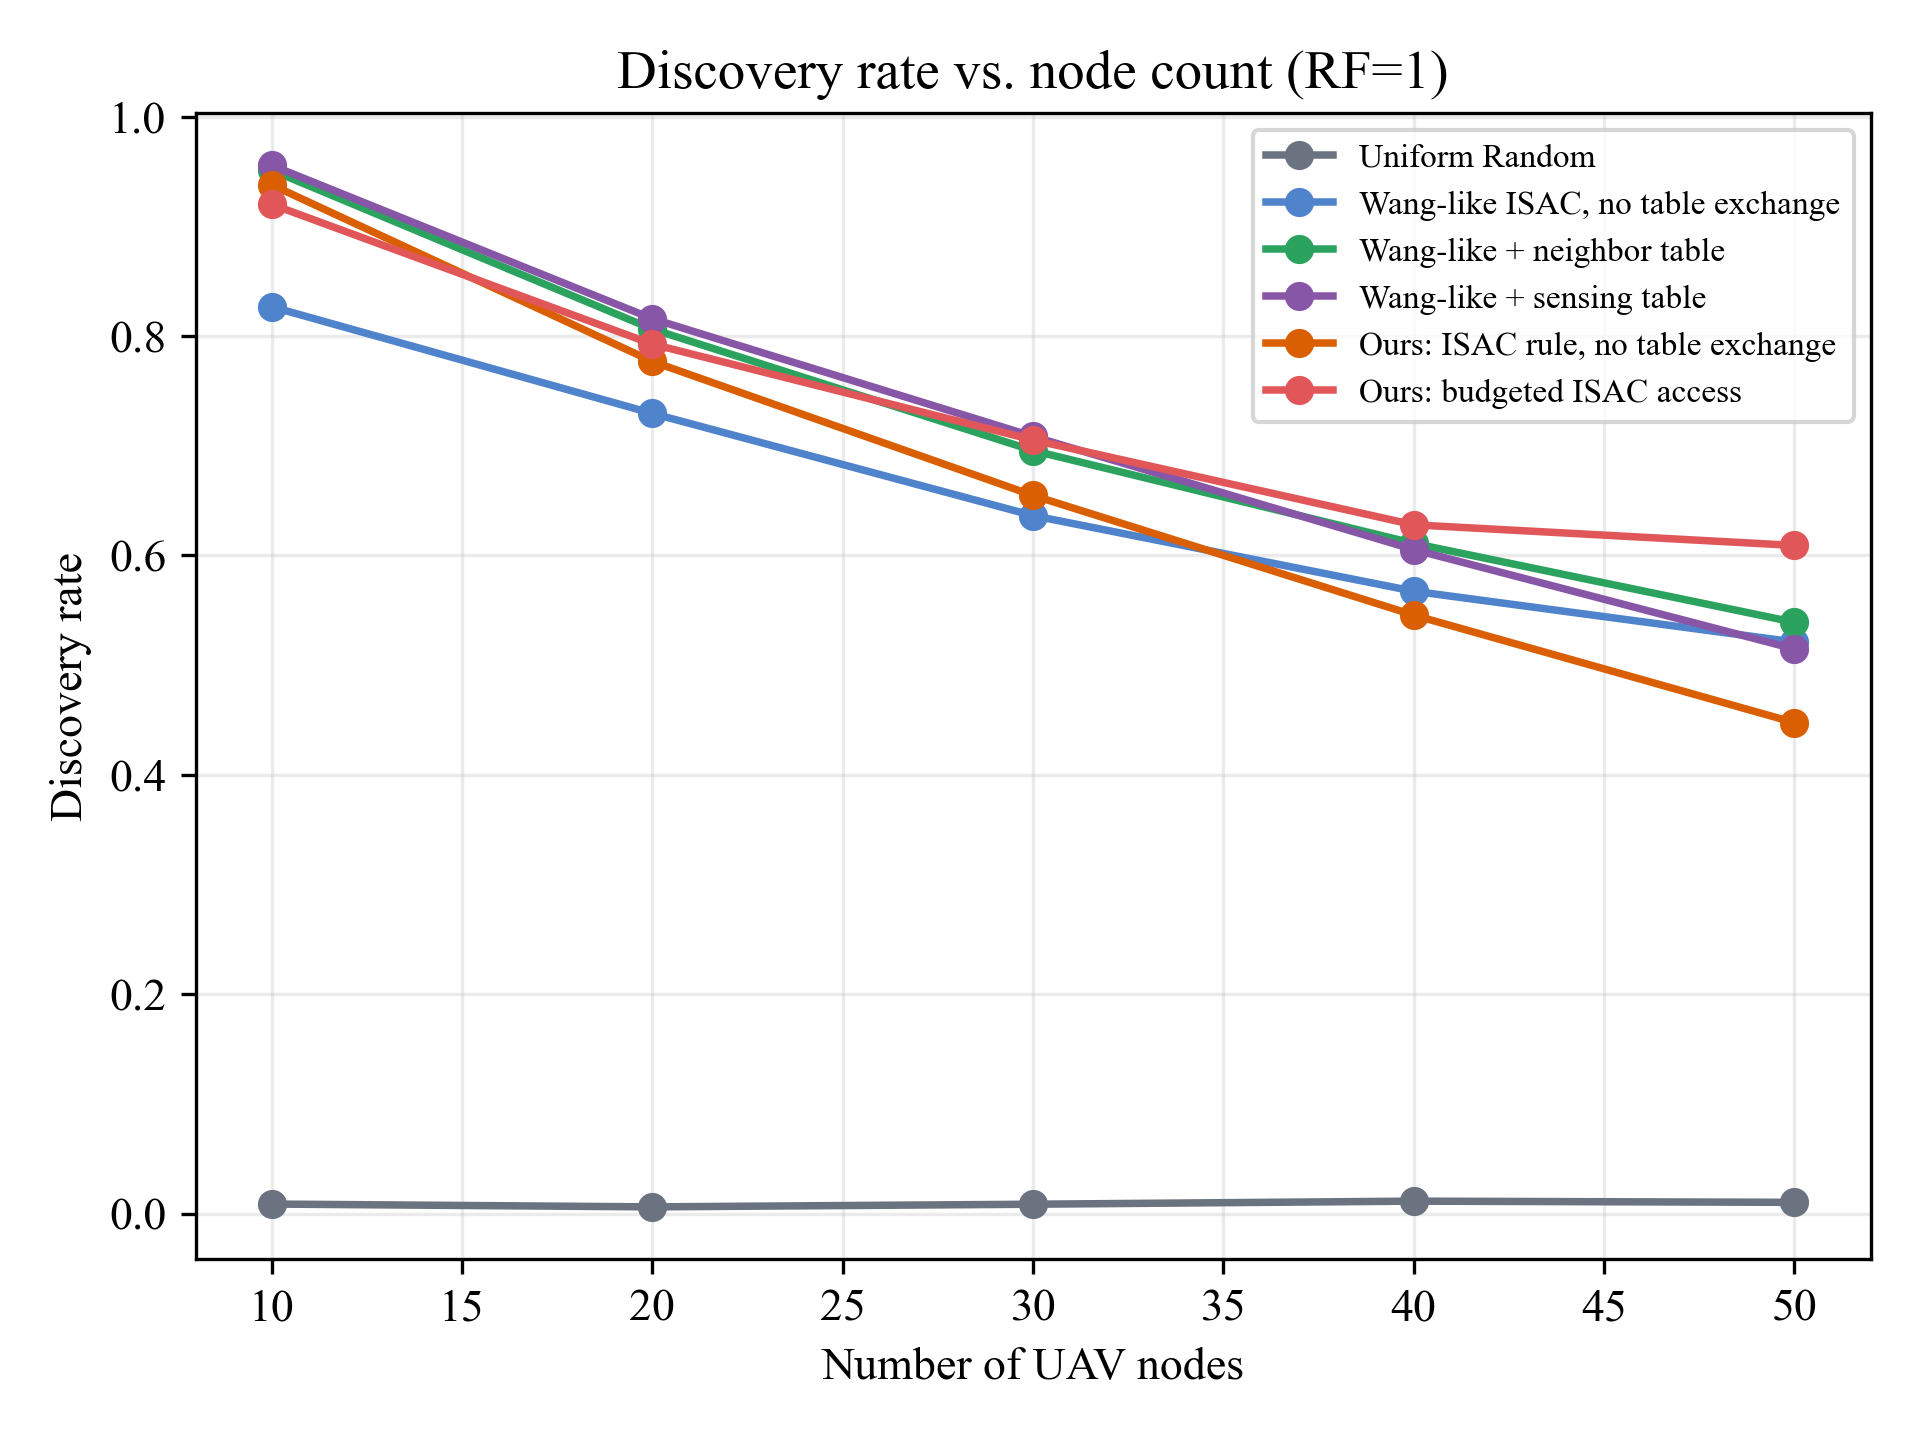
\includegraphics[width=\linewidth]{../../06_analysis/paper_figures/wang2025_focused_single_rf_20260709/node_scaling_discovery_rate_rf1.png}
  \caption{Finite-horizon discovery rate in the Wang-style single-RF matrix.}
  \label{fig:wang_focused_discovery}
\end{figure}

\begin{figure}[!t]
  \centering
  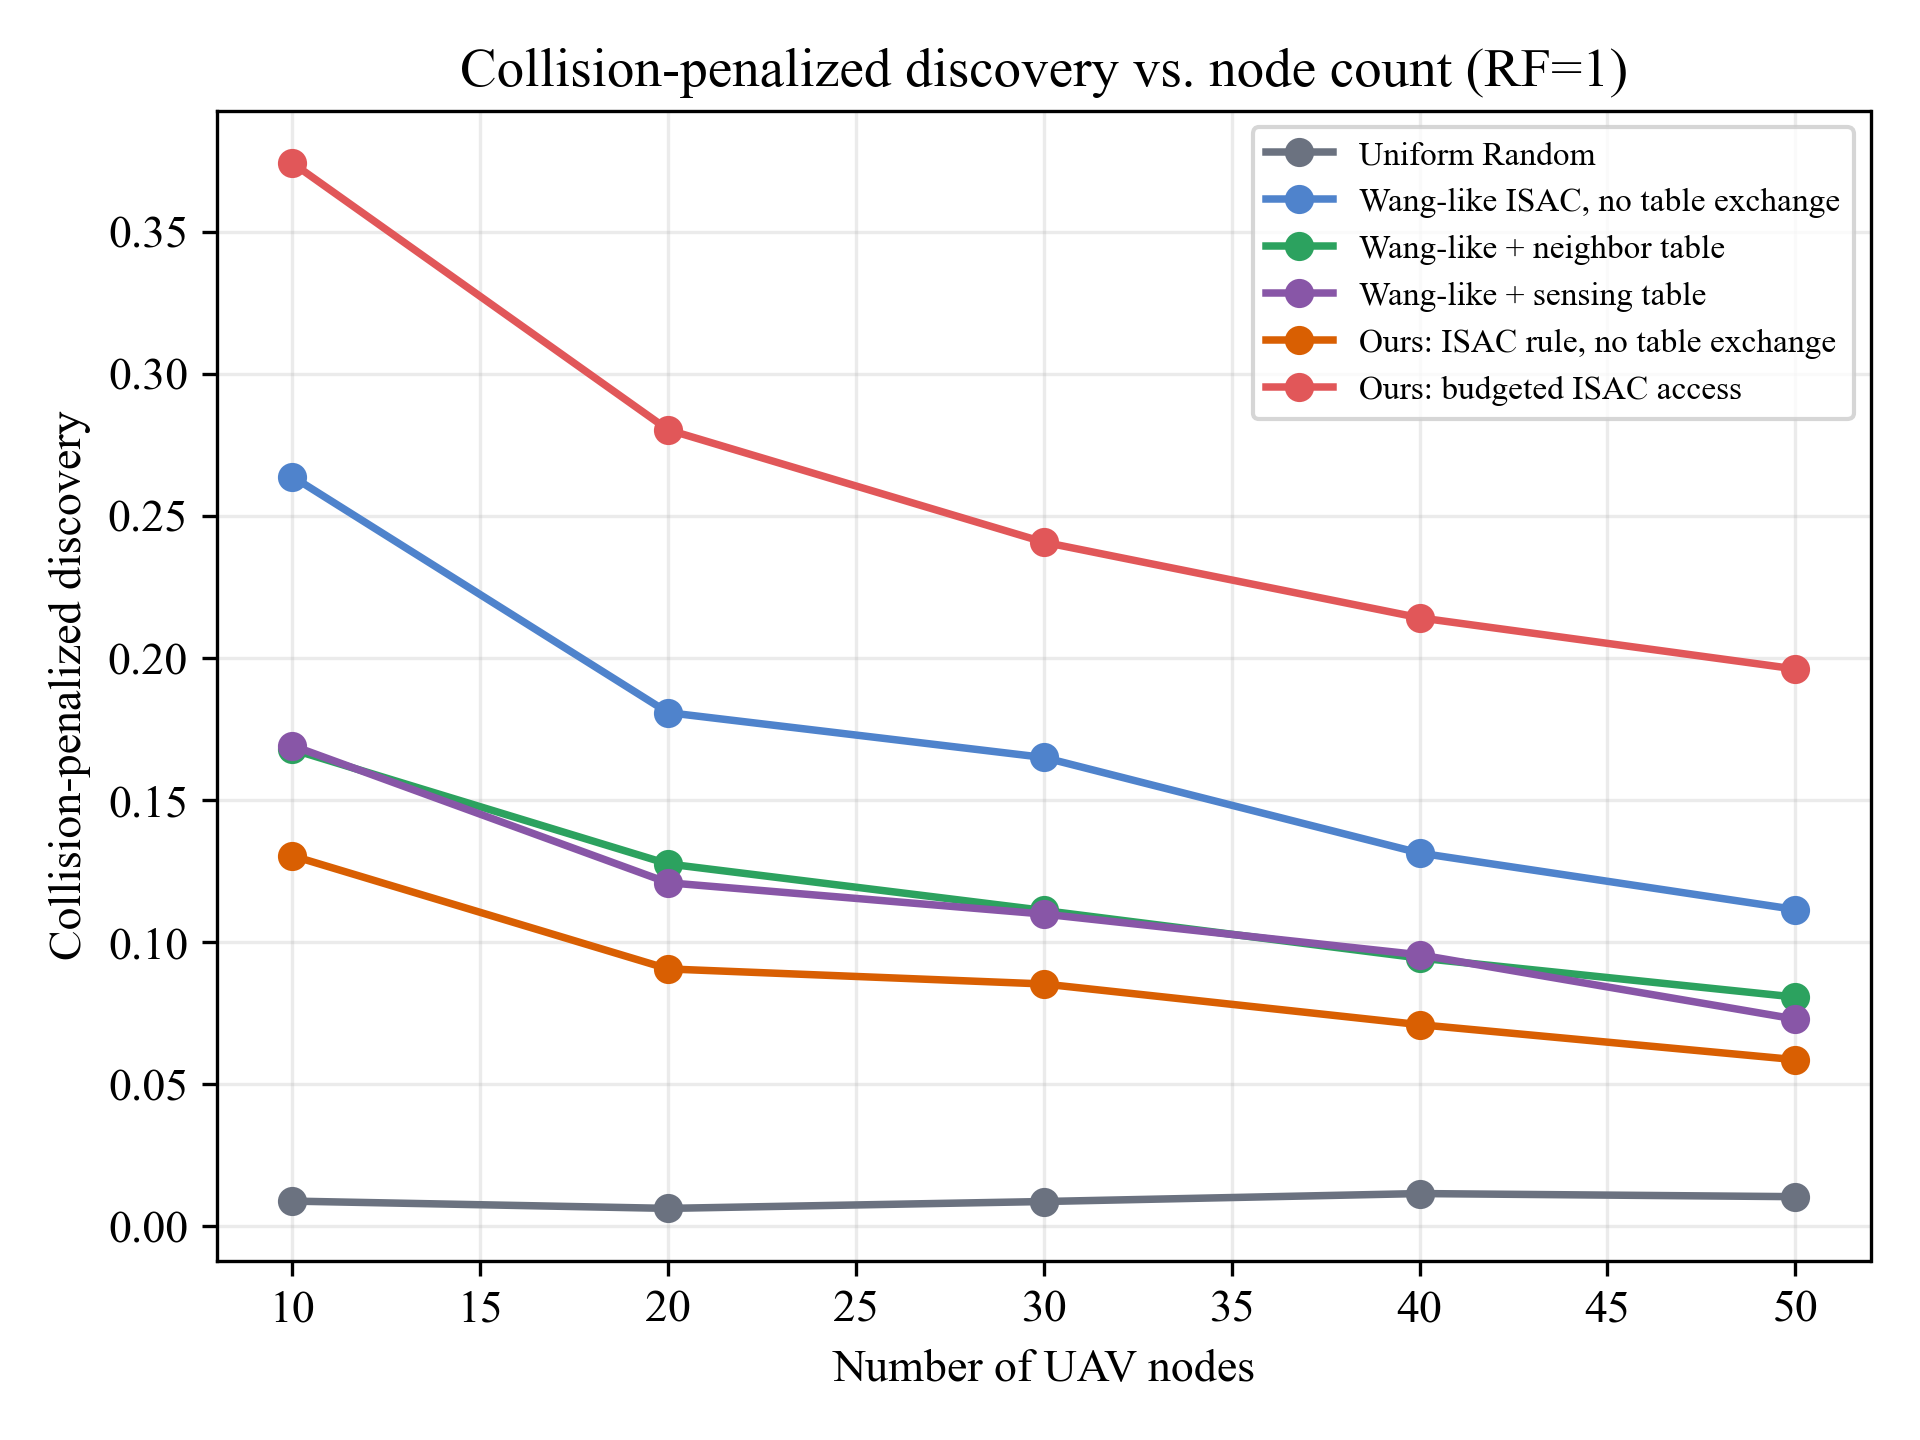
\includegraphics[width=\linewidth]{../../06_analysis/paper_figures/wang2025_focused_single_rf_20260709/node_scaling_cpd_rf1.png}
  \caption{Collision-penalized discovery in the Wang-style single-RF matrix.}
  \label{fig:wang_focused_cpd}
\end{figure}

\begin{table}[!t]
  \centering
  \caption{Focused Wang-Style Single-RF Results at \(N=50\)}
  \label{tab:wang_focused_n50}
  \begin{tabular}{lcccc}
    \toprule
    Protocol & Disc. & CPD & Coll. & \(\lambda_2\) \\
    \midrule
    Wang ISAC, no table & 0.5211 & 0.1115 & 4522.4 & 16.0628 \\
    Wang comm. table & 0.5391 & 0.0807 & 6999.4 & 17.6903 \\
    Wang sensing table & 0.5148 & 0.0729 & 7474.0 & 14.7000 \\
    Ours, non-budgeted ISAC & 0.4477 & 0.0587 & 8147.2 & 12.7513 \\
    Ours, budgeted ISAC & \textbf{0.6091} & \textbf{0.1961} & \textbf{2582.2} & \textbf{20.3632} \\
    \bottomrule
  \end{tabular}
\end{table}

The focused matrix shows that table exchange is not sufficient by itself under
dense single-RF access.  At \(N=50\), Wang-style sensing-table exchange reaches
discovery rate 0.5148 but incurs 7474.0 collisions, giving CPD 0.0729.  The
budgeted ISAC rule instead reaches discovery rate 0.6091 with 2582.2 collisions,
raising CPD to 0.1961 and \(\lambda_2\) to 20.3632.  Against the three
Wang-style baselines at \(N=50\), paired episode deltas are positive for
discovery and CPD, and negative for collisions, in all five episodes.  Compared
with the strongest Wang CPD baseline, the budgeted rule improves CPD by 0.0846
while also increasing discovery from 0.5211 to 0.6091.

These results support a narrower but cleaner cross-layer conclusion: under the
same ISAC sensing service abstraction, the main protocol gain comes from
collision-budgeted access to ISAC-suggested beams, not from unconstrained sharing
of neighbor or sensing tables.  The result should therefore be interpreted as a
link-layer budgeted access contribution built on top of ISAC sensing, rather
than as a new physical-layer MIMO-OTFS waveform design.
